\section{バンドパスフィルタ}


離散フーリエ変換によって算出された周波数領域のデータにおいて,ある範囲の
周波数成分のみを抽出し時間領域のデータに逆変換するフィルタ処理のことを
バンドパスフィルタという.
このとき,抽出する周波数成分の閾値のことをカットオフ周波数という.
バンドパスフィルタは,計測したデータにノイズが含まれている場合や任意の周波数を含む
信号のみを計測する場合などに活用される.
\autoref{fig:band_pass}, \autoref{fig:band_ipass}にバンドパスフィルタを\autoref{fig:digital_sin}に対して行った例を示す.
\autoref{fig:band_pass}では,バンドパスフィルタを用いて$3 \le \omega \le 7$の周波数を抽出しており,
\autoref{fig:band_ipass}において6Hzのみのデータが抽出できていることがわかる.

\iffigure
\begin{figure}[h]
    \centering
  \begin{minipage}{.45\hsize}
    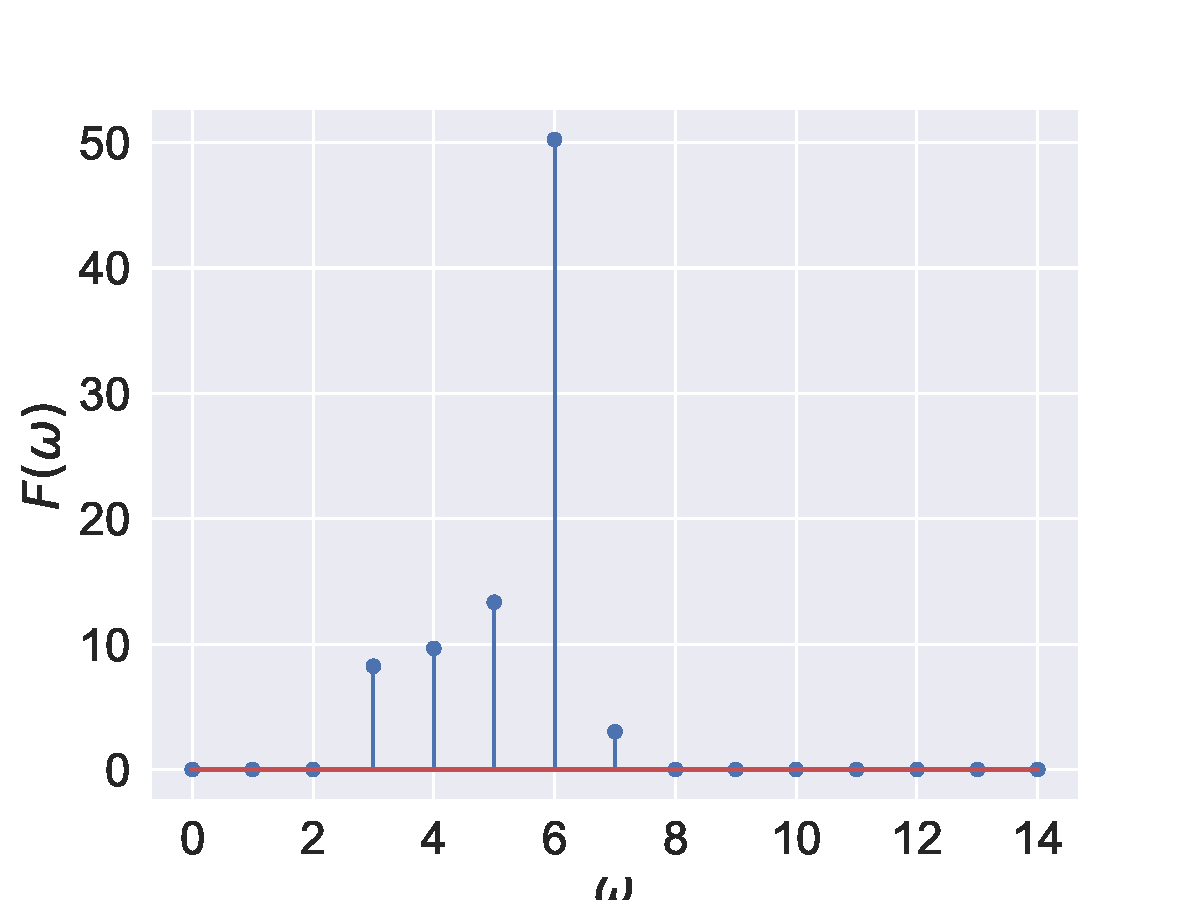
\includegraphics[clip, width=\textwidth]{figure/band_pass_dft.pdf}
    \caption{\autoref{fig:dft}に対してバンドパスフィルタを行った場合(周波数領域)}
    \label{fig:band_pass}
  \end{minipage}
  \begin{minipage}{.45\hsize}
    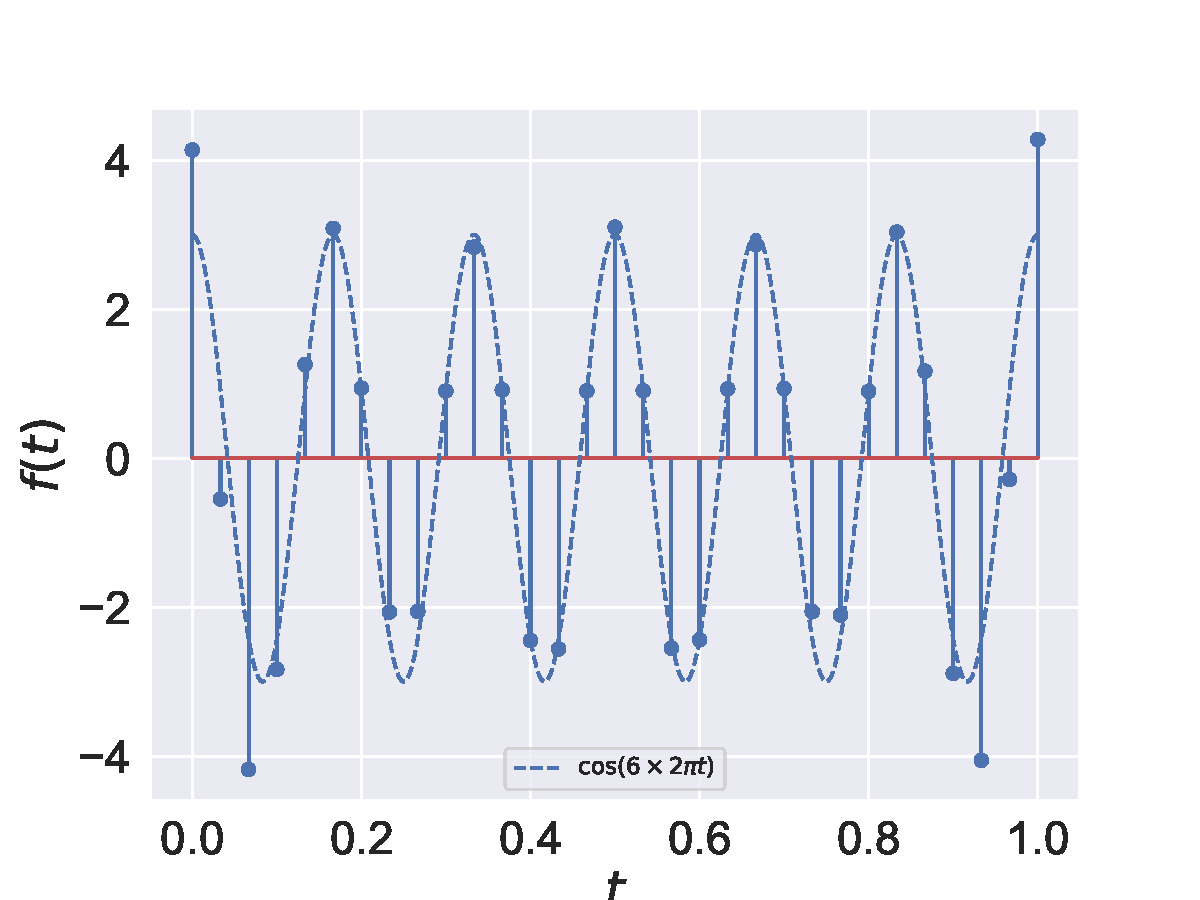
\includegraphics[clip, width=\textwidth]{figure/band_pass_idft.pdf}
    \caption{\autoref{fig:dft}に対してバンドパスフィルタを行った場合(時間領域)}
    \label{fig:band_ipass}
  \end{minipage}
\end{figure}
\fi
バンドパスフィルタにおいて,単一のカットオフ周波数以上の範囲のみを
抽出し高周波領域のデータを抽出するフィルタ処理をハイパスフィルタという.
\autoref{fig:band_pass}, \autoref{fig:band_ipass}にハイパスフィルタを\autoref{fig:digital_sin}に対して行った例を示す.
\autoref{fig:band_pass}では,ハイパスフィルタを用いて$7 \le \omega \le 14$の周波数を抽出しており,
\autoref{fig:band_ipass}において10Hzのみのデータが抽出できていることがわかる.

\iffigure
\begin{figure}[h]
    \centering
  \begin{minipage}{.45\hsize}
    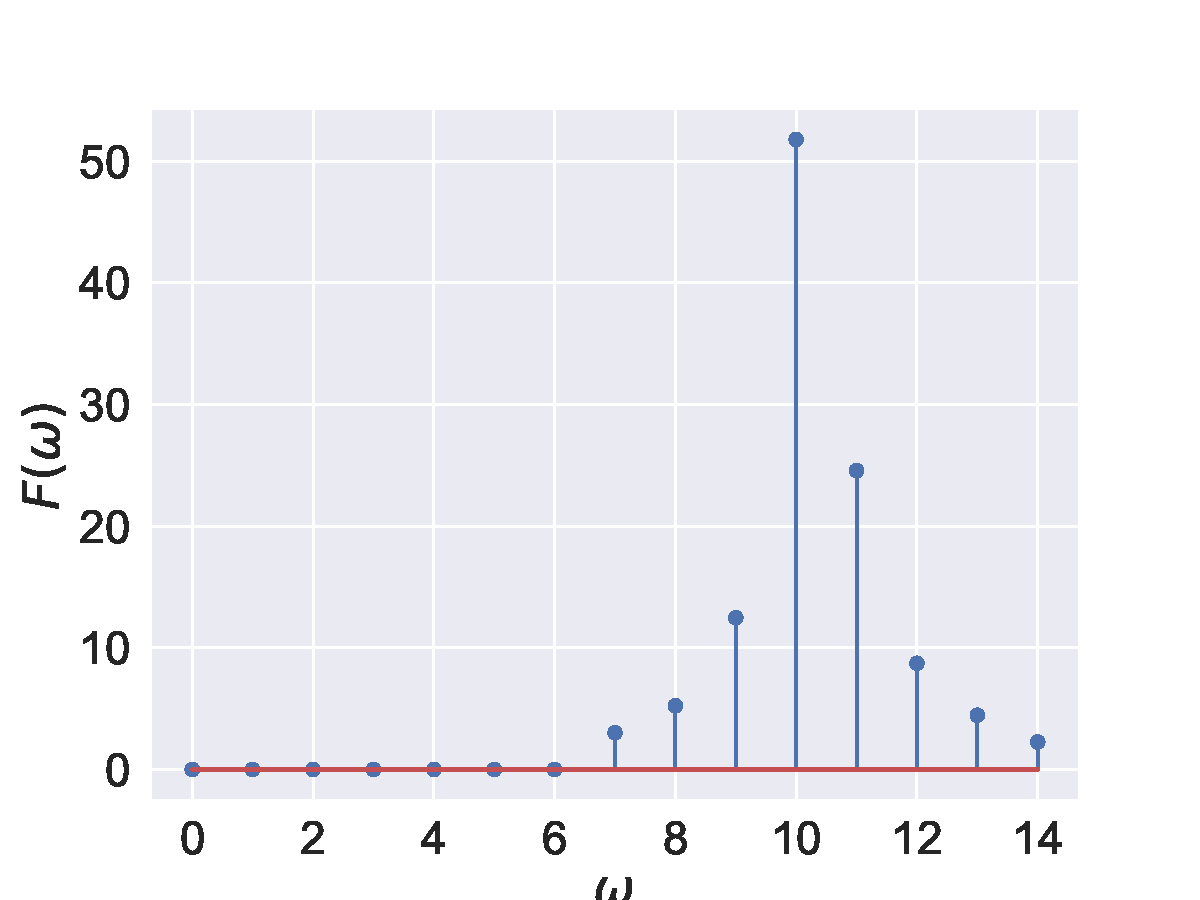
\includegraphics[clip, width=\textwidth]{figure/high_pass_dft.pdf}
    \caption{\autoref{fig:dft}に対してハイパスフィルタを行った場合(周波数領域)}
    \label{fig:high_sin}
  \end{minipage}
  \begin{minipage}{.45\hsize}
    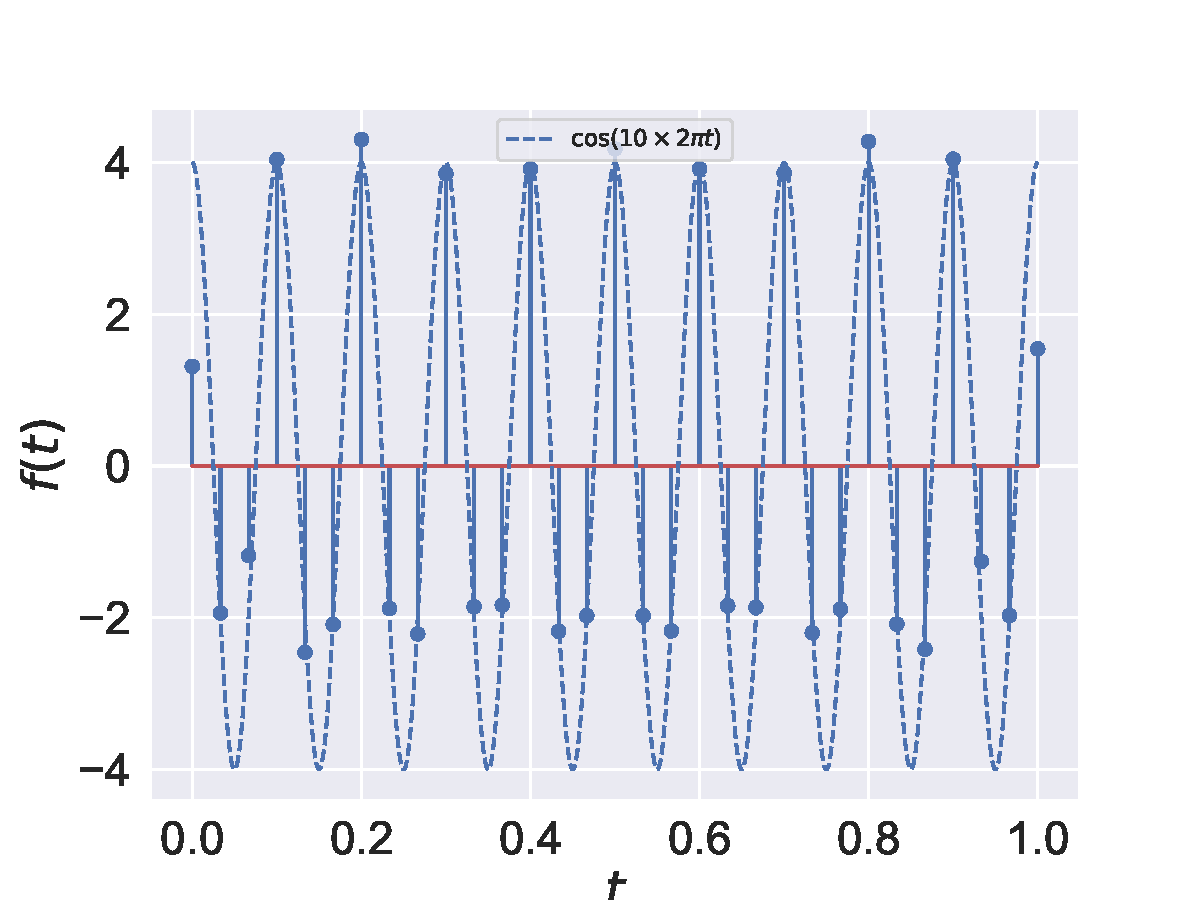
\includegraphics[clip, width=\textwidth]{figure/high_pass_idft.pdf}
    \caption{\autoref{fig:dft}に対してハイパスフィルタを行った場合(時間領域)}
    \label{fig:high_sin}
  \end{minipage}
\end{figure}
\fi

また,カットオフ周波数以下の範囲のみを
抽出し高周波領域のデータを抽出するフィルタ処理をローパスフィルタという.
\autoref{fig:low_pass}, \autoref{fig:low_ipass}にローパスフィルタを\autoref{fig:digital_sin}に対して行った例を示す.
\autoref{fig:low_pass}では,バンドパスフィルタを用いて$0 \le \omega \le 3$の周波数を抽出しており,
\autoref{fig:low_ipass}において1Hzのみのデータが抽出できていることがわかる.

\iffigure
\begin{figure}[h]
    \centering
  \begin{minipage}{.45\hsize}
    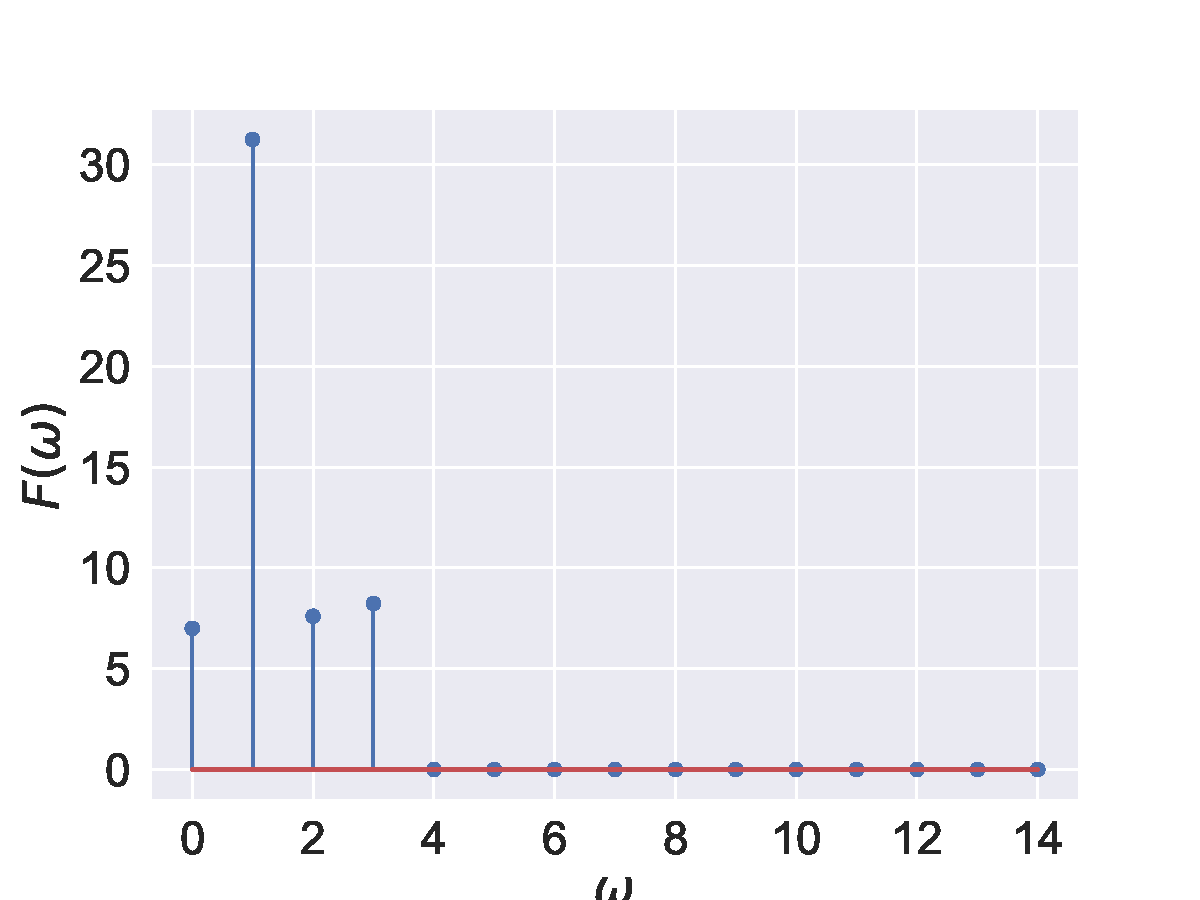
\includegraphics[clip, width=\textwidth]{figure/low_pass_dft.pdf}
    \caption{\autoref{fig:dft}に対してローパスフィルタを行った場合(周波数領域)}
    \label{fig:low_pass}
  \end{minipage}
  \begin{minipage}{.45\hsize}
    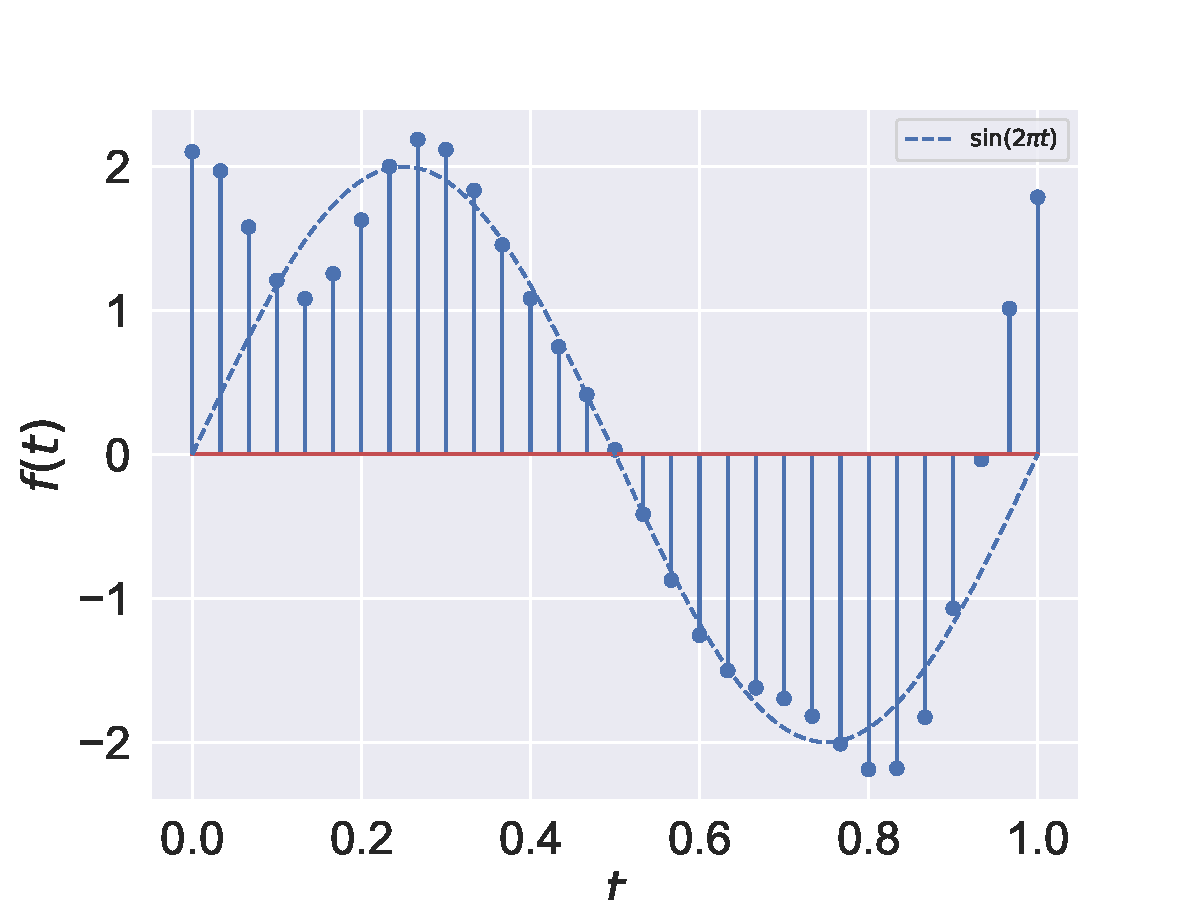
\includegraphics[clip, width=\textwidth]{figure/low_pass_idft.pdf}
    \caption{\autoref{fig:dft}に対してローパスフィルタを行った場合(時間領域)}
    \label{fig:low_ipass}
  \end{minipage}
\end{figure}
\fi
